
\documentclass[xcolor={dvipsnames}]{beamer}
\usepackage{amsmath,amsfonts,amssymb,pxfonts,eulervm,xspace}
\usepackage{tabularx}
\usepackage{multirow}
\usepackage{graphicx}


\graphicspath{.figs/}

\usepackage[backend=bibtex, style=numeric-comp, doi=false,isbn=false,url=false, giveninits=true]{biblatex}
\bibliography{../paper/main.bib}

\usetheme{ccnycrest}


\newenvironment{changemargin}[2]{%
\begin{list}{}{%
\setlength{\topsep}{0pt}%
\setlength{\leftmargin}{#1}%
\setlength{\rightmargin}{#2}%
\setlength{\listparindent}{\parindent}%
\setlength{\itemindent}{\parindent}%
\setleng{}th{\parsep}{\parskip}%
}%
\item[]}{\end{list}}

\begin{document}

\title{Visualizing Conditional Dependencies}

\begin{frame}
	\titlepage
    Hannah Aizenman\\
    Advisor: Dr. Michael Grossberg \\
    Committee: Dr. Robert Haralick, Dr. Lev Manovich, Dr. Huy Vo\\
\end{frame}

\begin{frame}{Predictions are Uncertain}
\begin{figure}
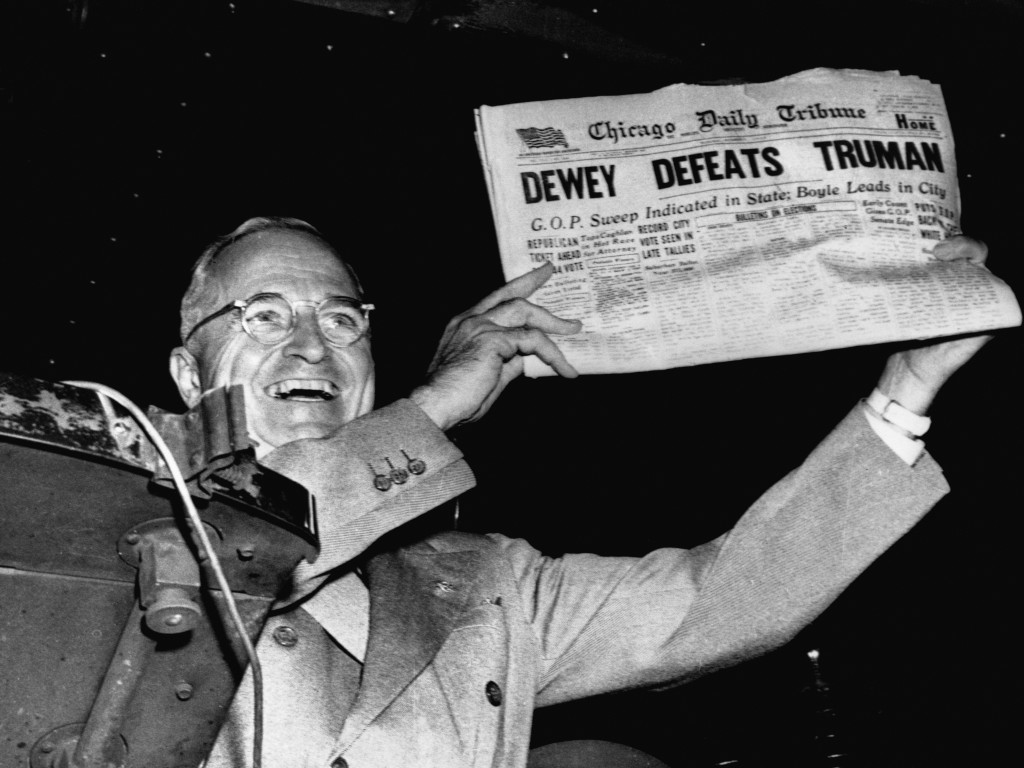
\includegraphics[width=\textwidth]{figs/gettyimages-517387760.jpg}
\end{figure}
\end{frame}

\begin{frame}{So Let's Incorporate Uncertainty}
\begin{figure}
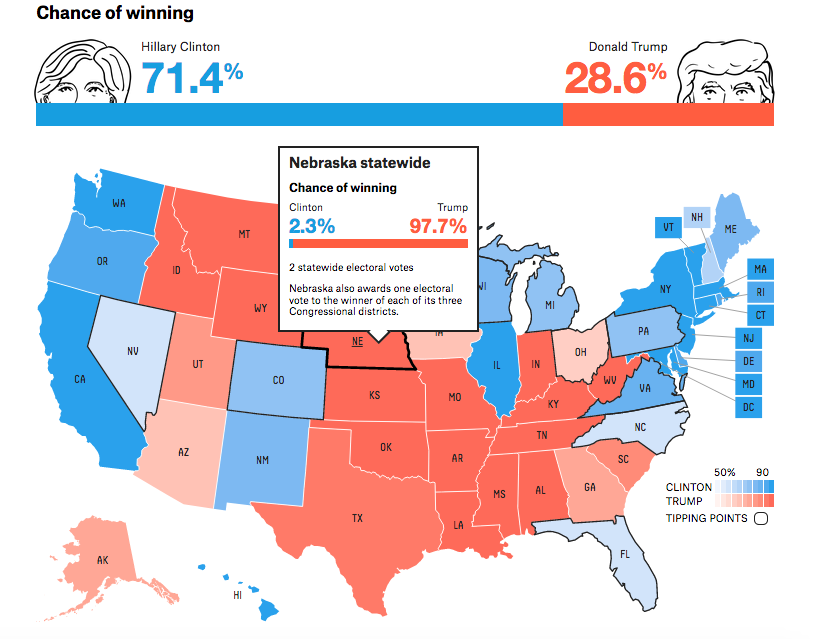
\includegraphics[width=\textwidth]{figs/fivethirtyeight.png}
\end{figure}
\end{frame}

\begin{frame}{But What About Observations?}
\begin{figure}
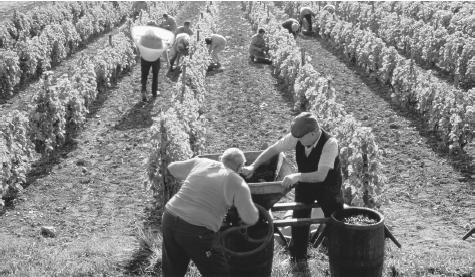
\includegraphics[width=\textwidth]{figs/ctc_02_img0397.jpg}
\end{figure}
\end{frame}

\begin{frame}{Bertin's 1954 French Workforce\cite{bertin_semiology_2011}}
\begin{itemize}
    \item Geographic region of France
    \item Number of employees (per thousand)
    \item Employment sector: agriculture, industry, everything else
\end{itemize}
\end{frame}

\begin{frame}{What questions are we asking?}
\begin{figure}
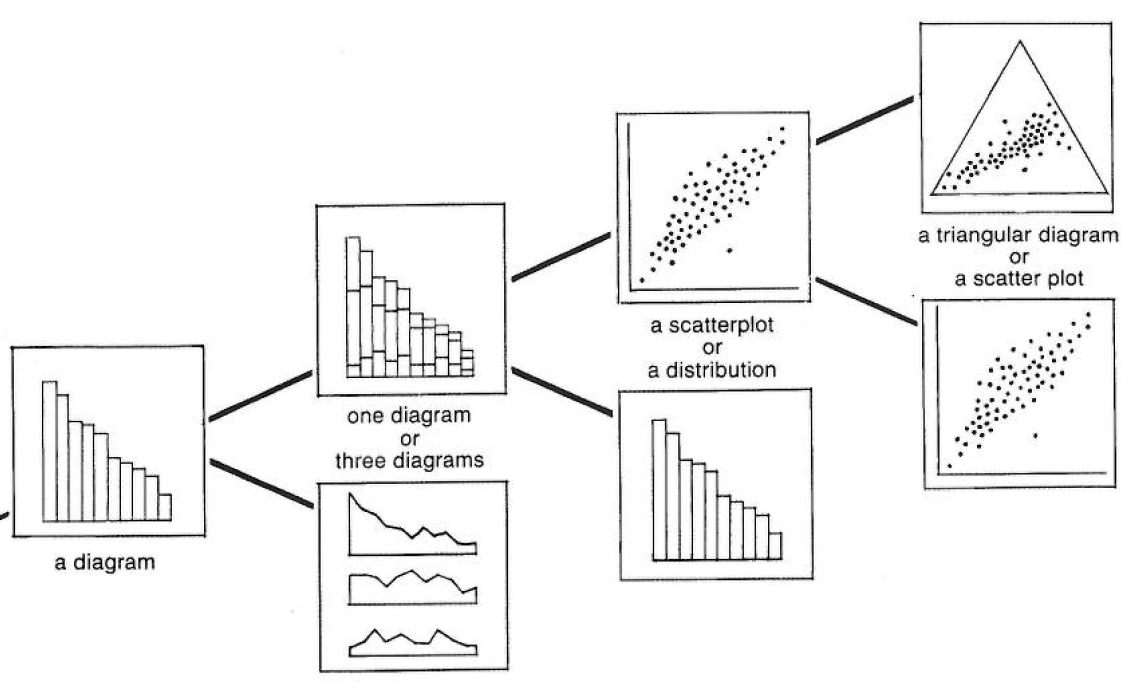
\includegraphics[width=\textwidth]{figs/chart_chooser_top.png}
\end{figure}
\end{frame}

\begin{frame}{Incorporate geographic information?}
\begin{figure}
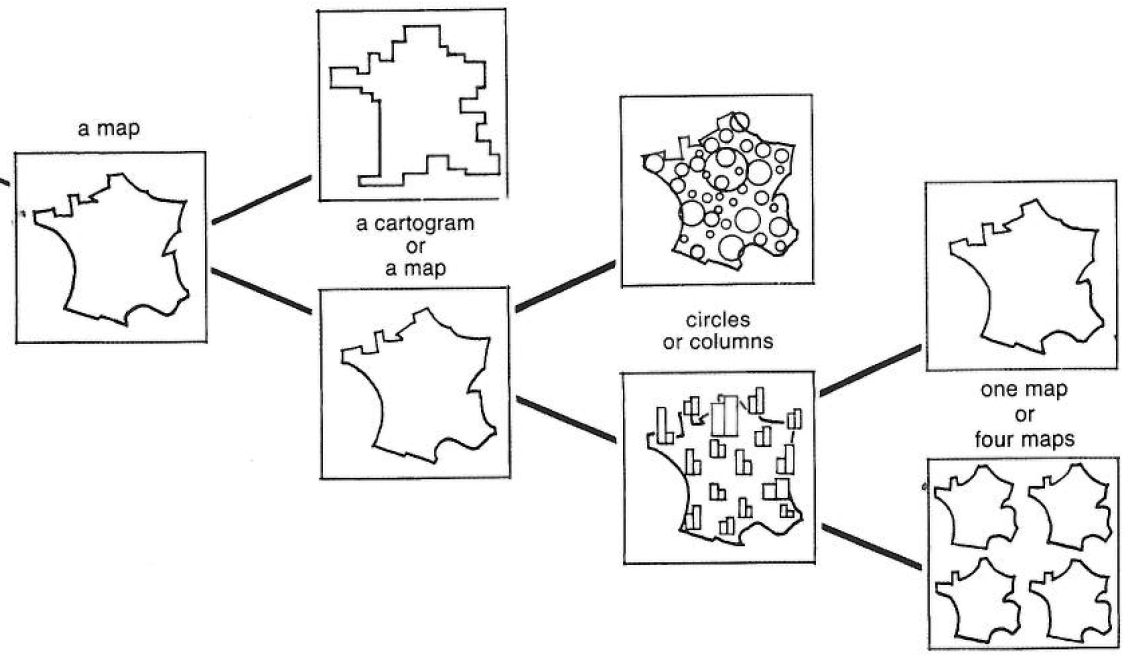
\includegraphics[width=\textwidth]{figs/chart_chooser_bottom.png}
\end{figure}
\end{frame}

\begin{frame}{What if we had more data?}
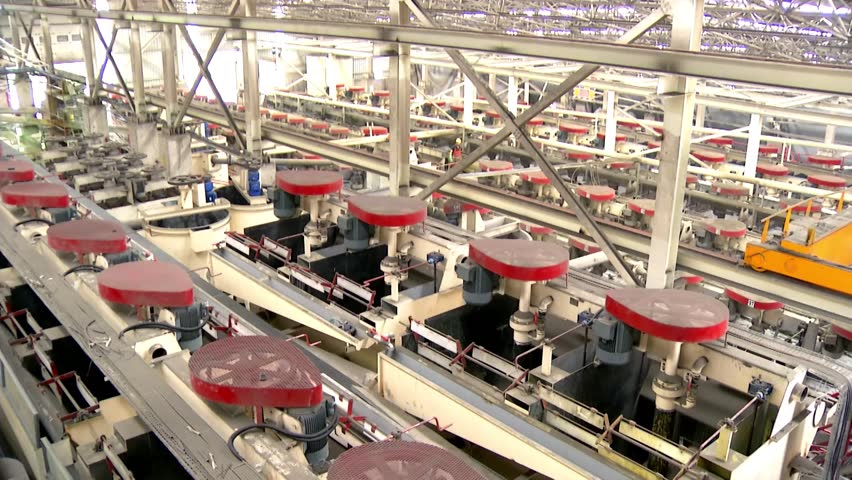
\includegraphics[width=\textwidth]{figs/growingeconomy.jpg}
\end{frame}

\begin{frame}
{\huge
\begin{align*}
P(v_1, v_2,...v_n \mid k_1, k_2,...k_n)
\end{align*}
}
\begin{block}{Extending Munzner's Keys \& Values \cite{munzner_what:_2014}}
    \begin{description}
        \item[value] unknown distribution/density
        \item[key] known look up measurement 
    \end{description}
\end{block}
\end{frame}


\begin{frame}{Apply this framework to data?}
\begin{block}{What's the likelihood of employment in each sector in Paris?}
    \begin{description}
        \item[value] sector
        \item[keys] region=Lyon
    \end{description}
\end{block}

\pause
\begin{block}{How are transportation workers distributed across France?}
    \begin{description}
        \item[values] region
        \item[key] sector=transportation
    \end{description}
\end{block}
\end{frame}

\begin{frame}{Ordering Visualizations by Keys and Values}
\begin{figure}
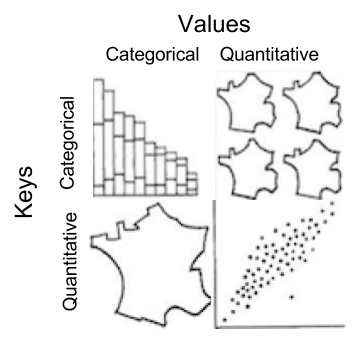
\includegraphics[height=.75\textheight]{figs/bertinf.png}
\end{figure}
\end{frame}

\section{Categorical Keys and Categorical Values}
\frame{\sectionpage}

\begin{frame}{Star Wars Super Graphic\cite{leong_star_2017}}
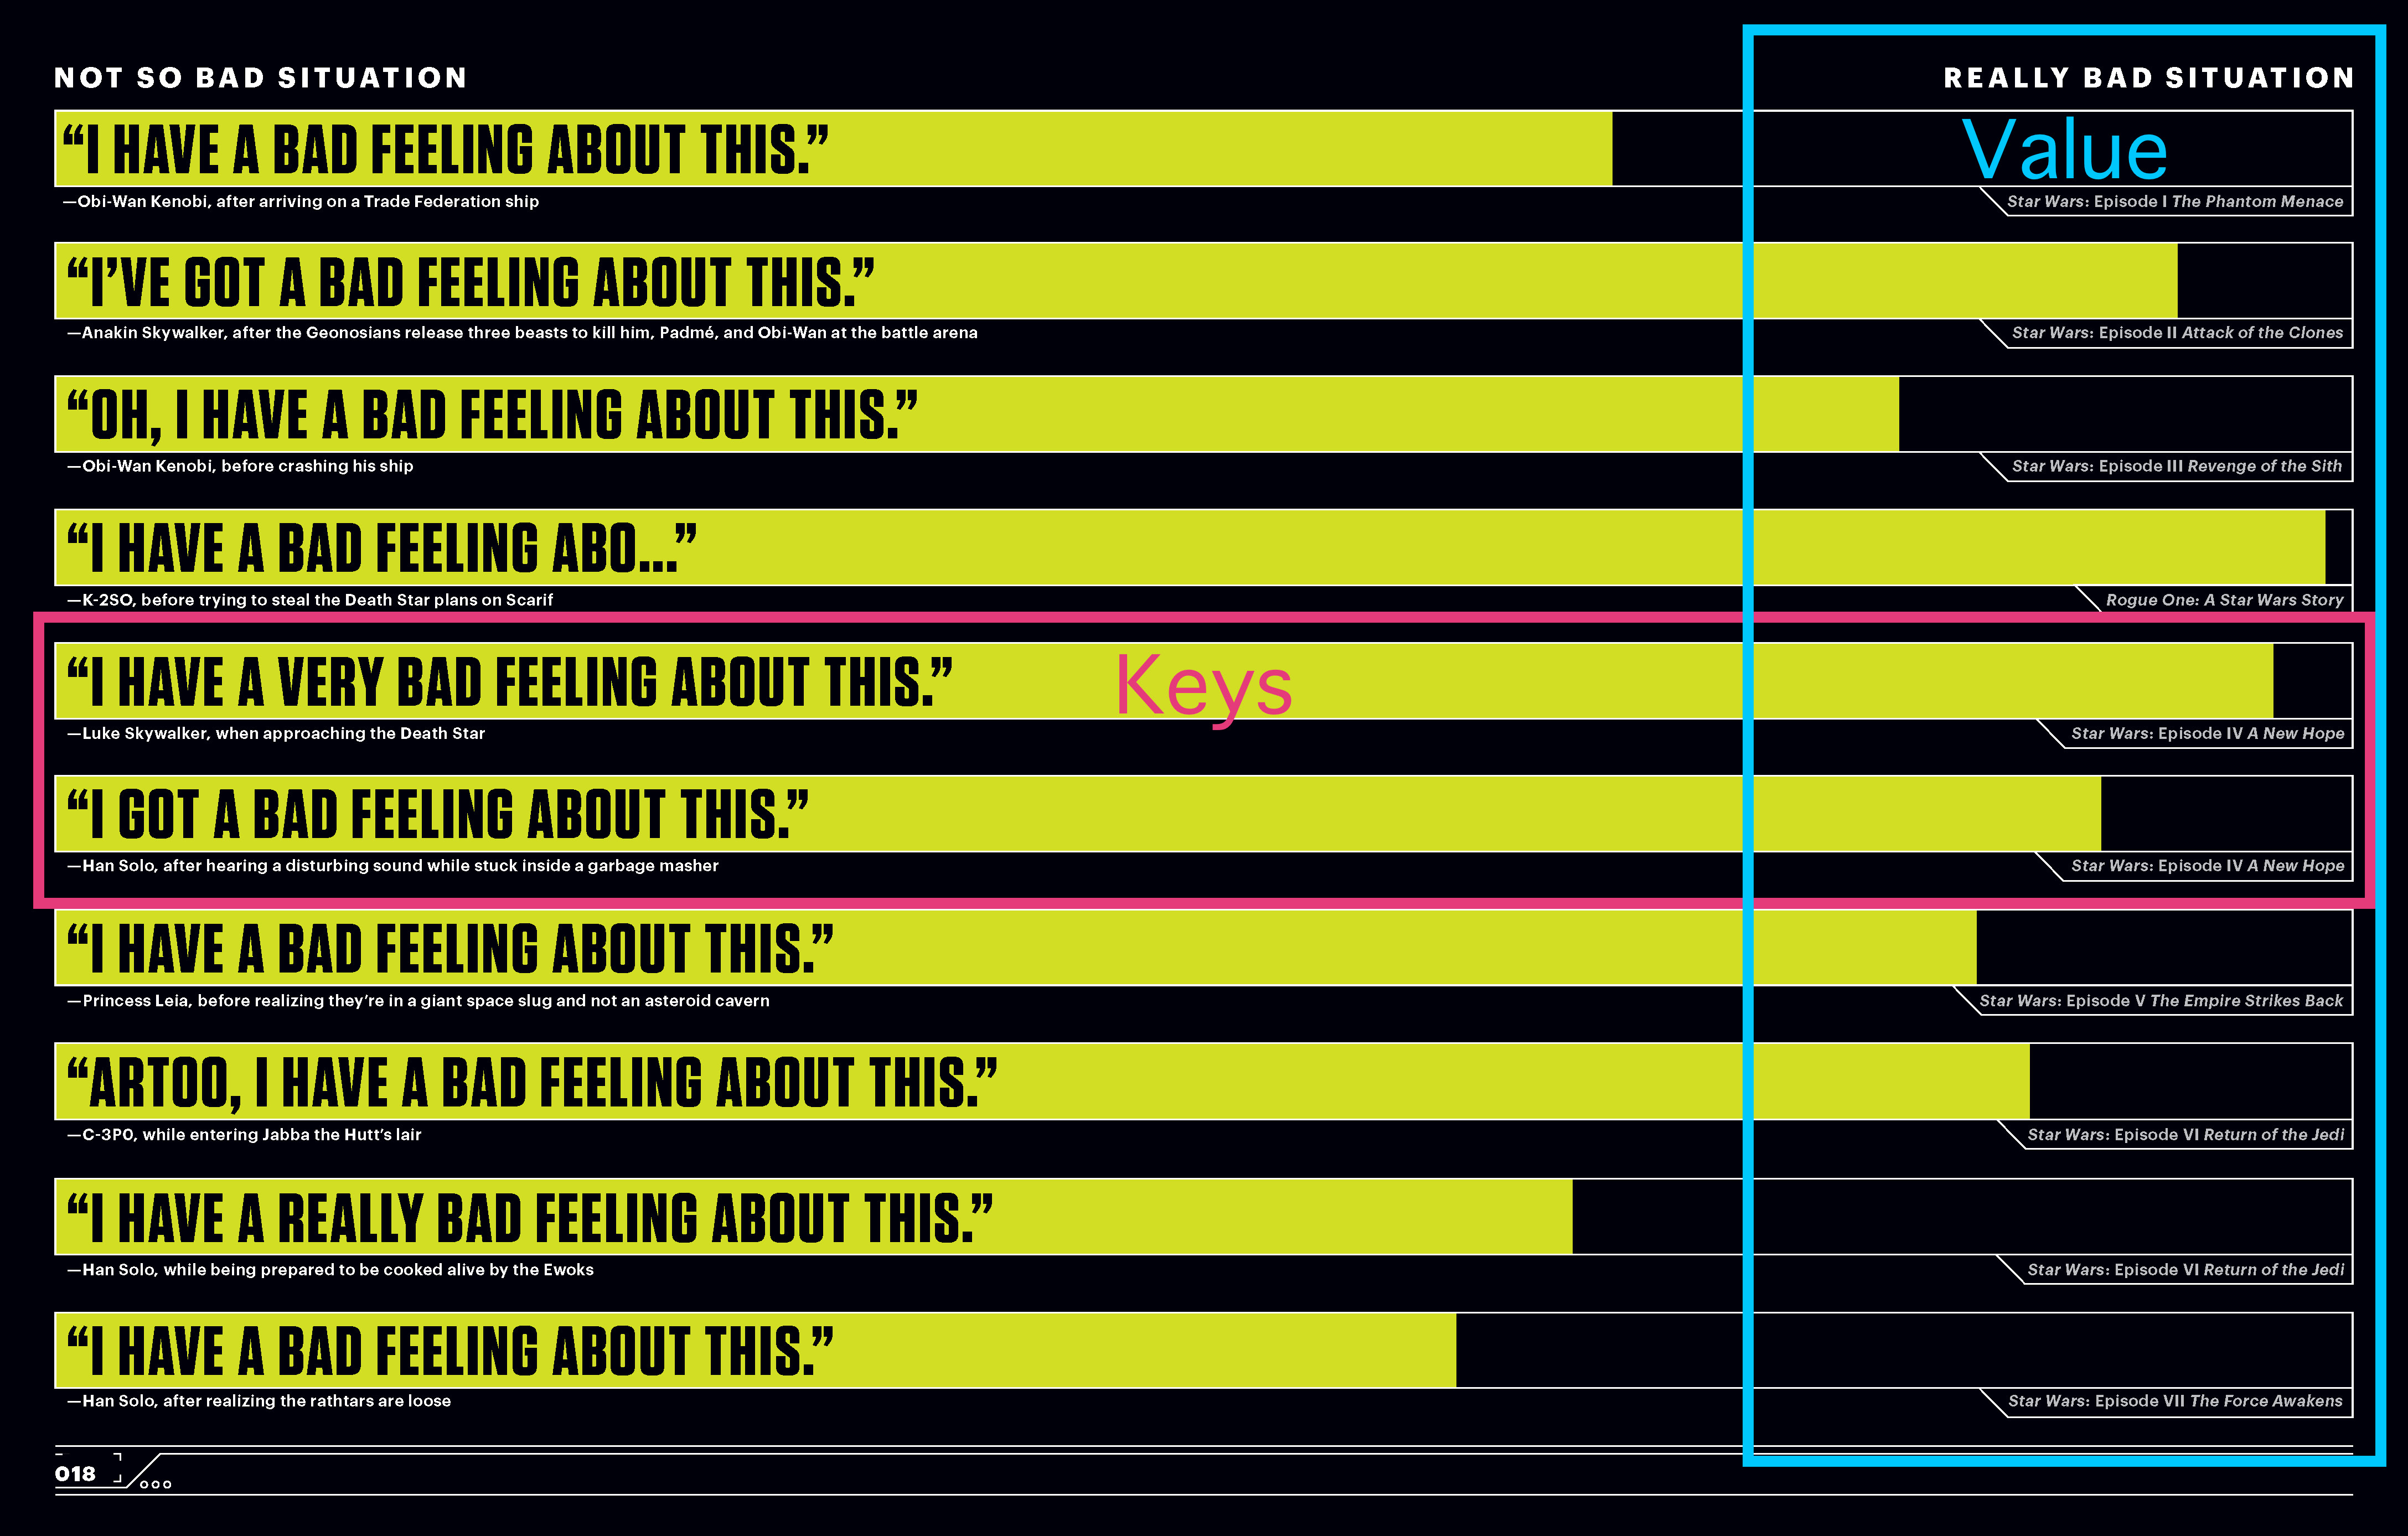
\includegraphics[width=\textwidth]{figs/starwards.jpeg}
\end{frame}

\begin{frame}{Parallel Sets\cite{kosara_parallel_2006}}
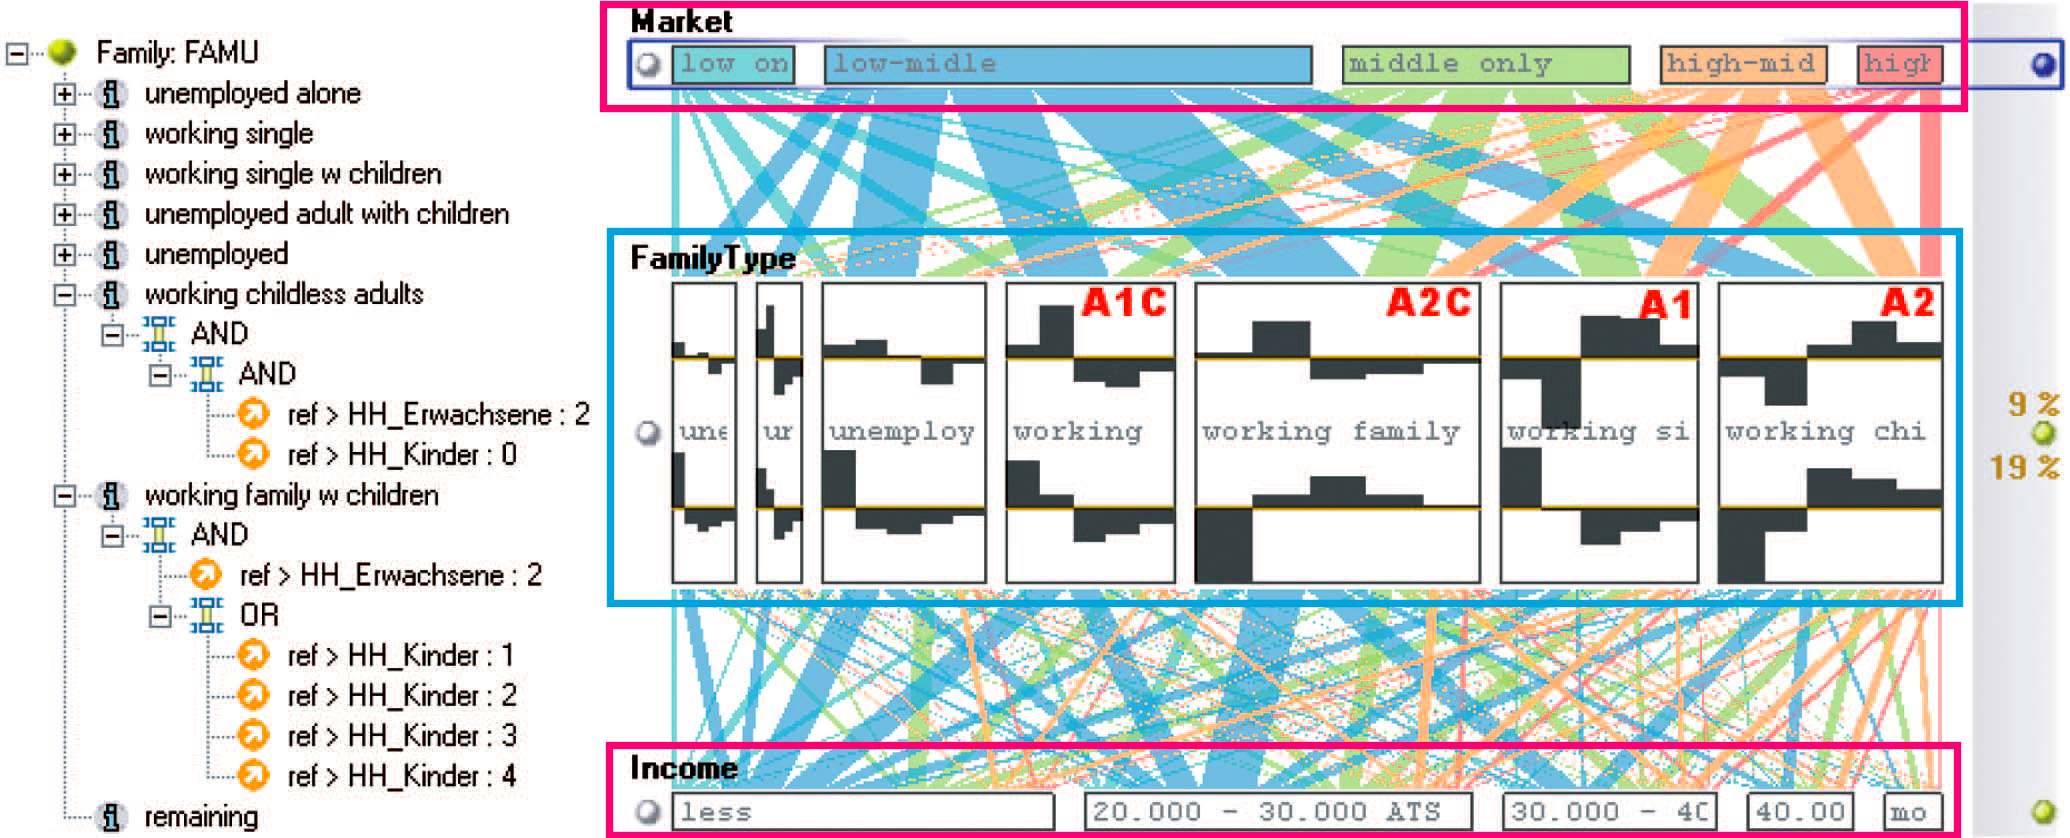
\includegraphics[width=\textwidth]{figs/parallelsets.png}
\end{frame}


\begin{frame}{Radar Chart \cite{albo_off_2016}}
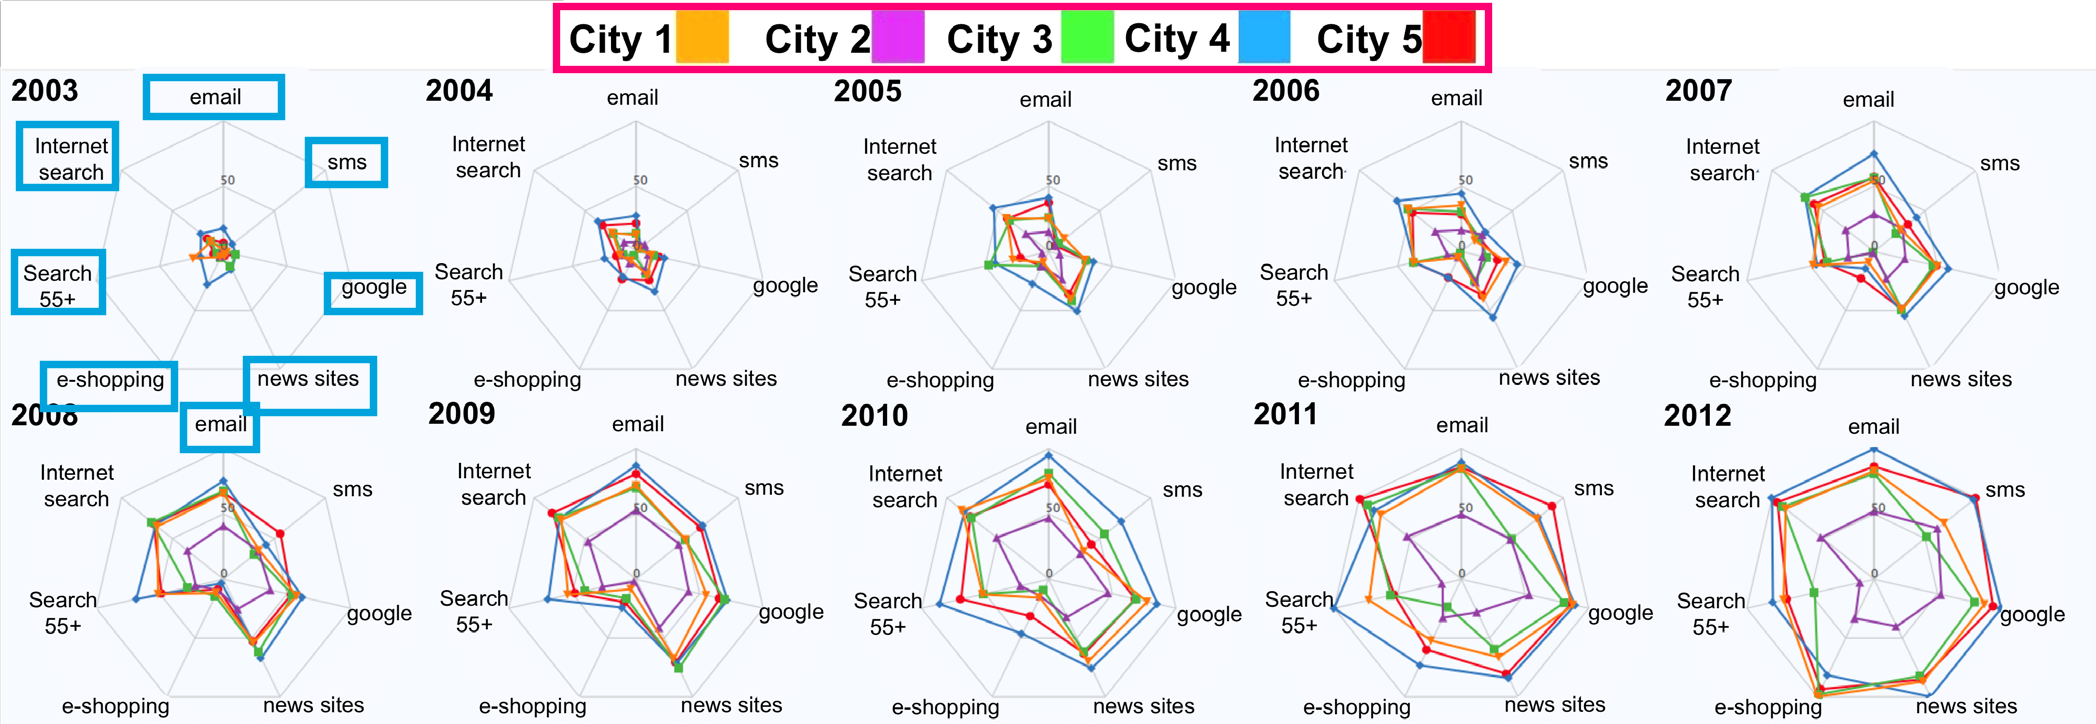
\includegraphics[width=\textwidth]{figs/cities_anotated.png}
\end{frame}

\begin{frame}{Flower Chart \cite{albo_off_2016}}
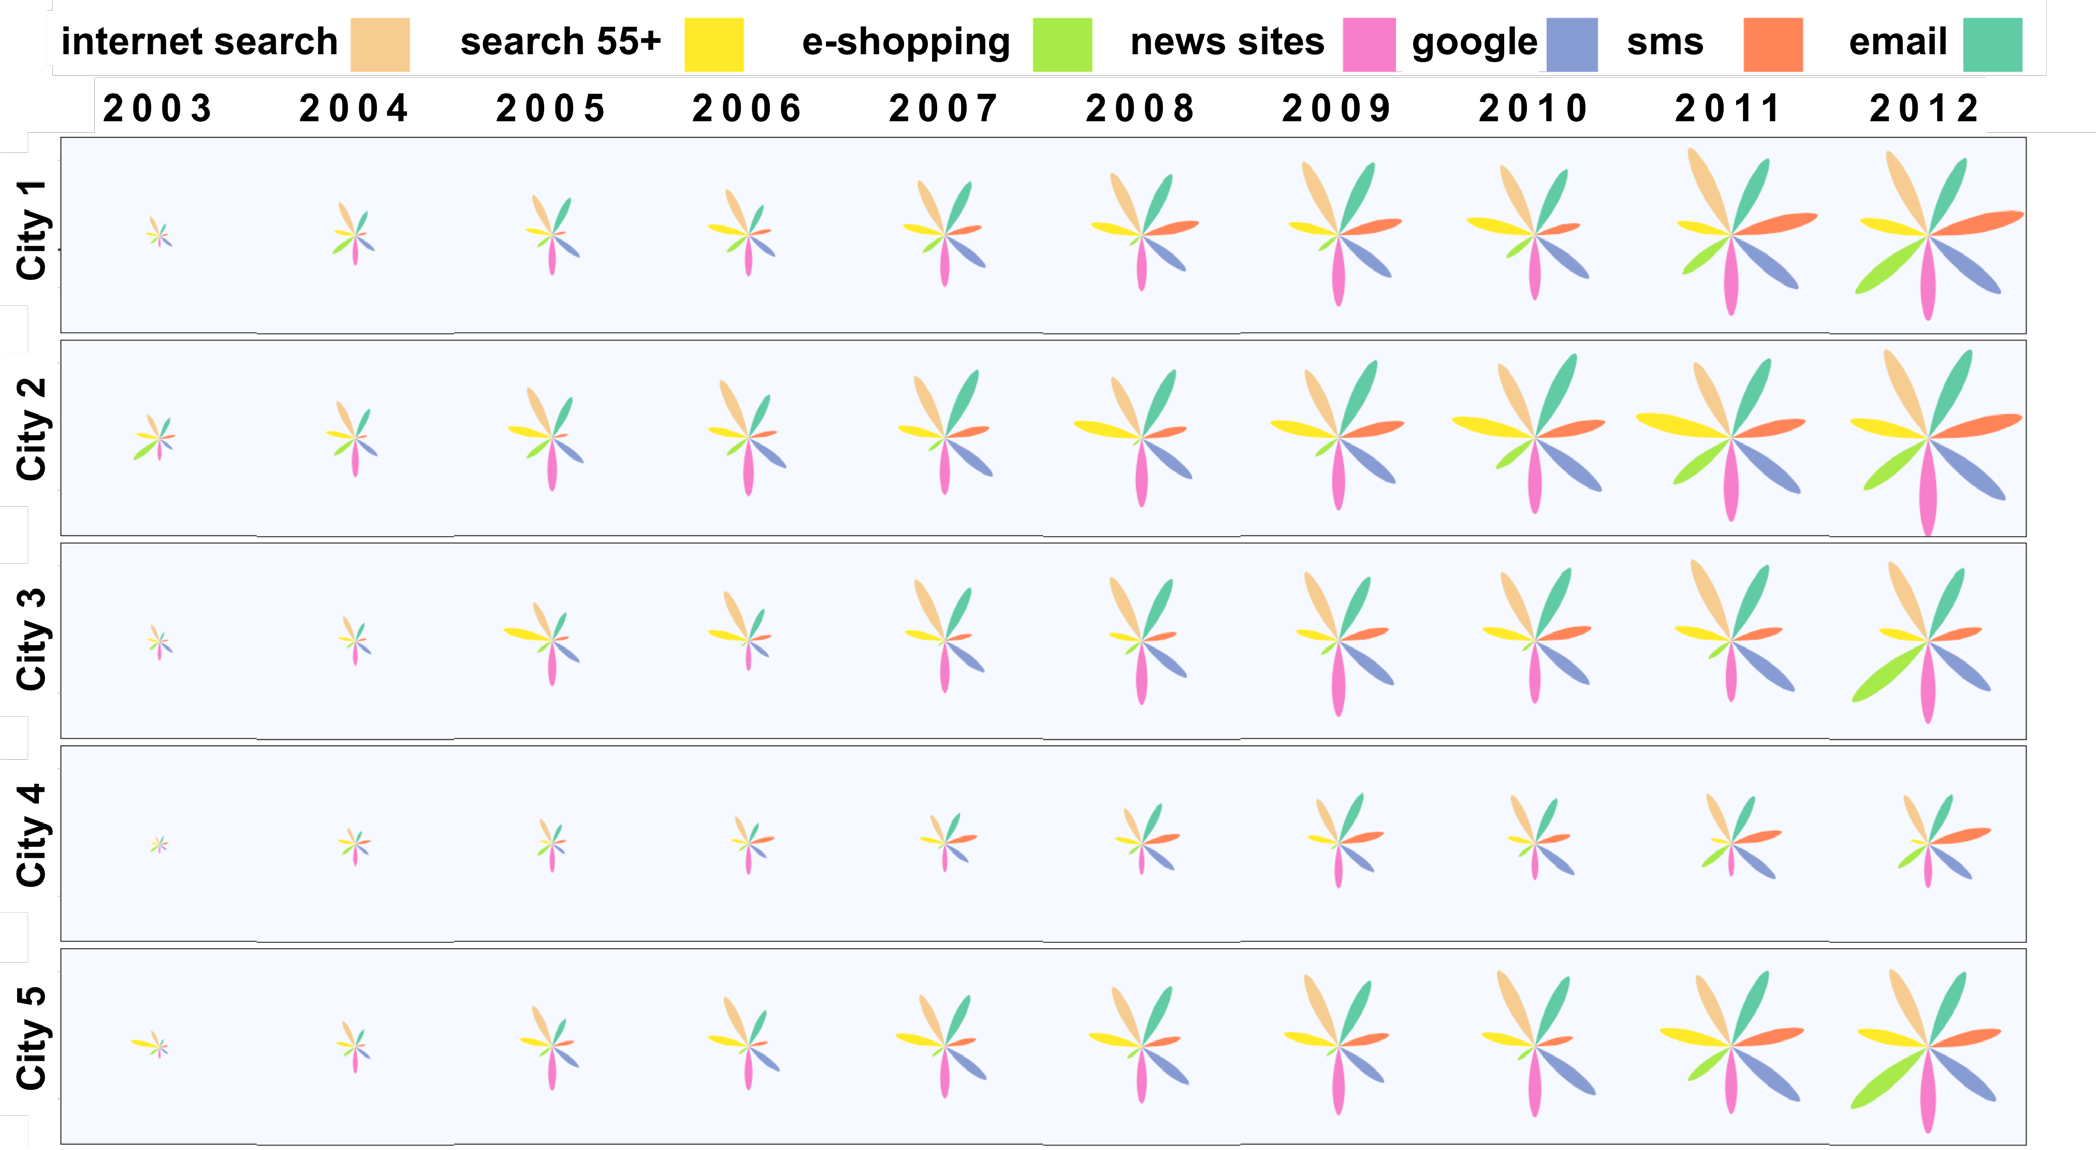
\includegraphics[width=\textwidth]{figs/flower_anotated.png}
\end{frame}

\begin{frame}{Circle Chart\cite{albo_off_2016}}
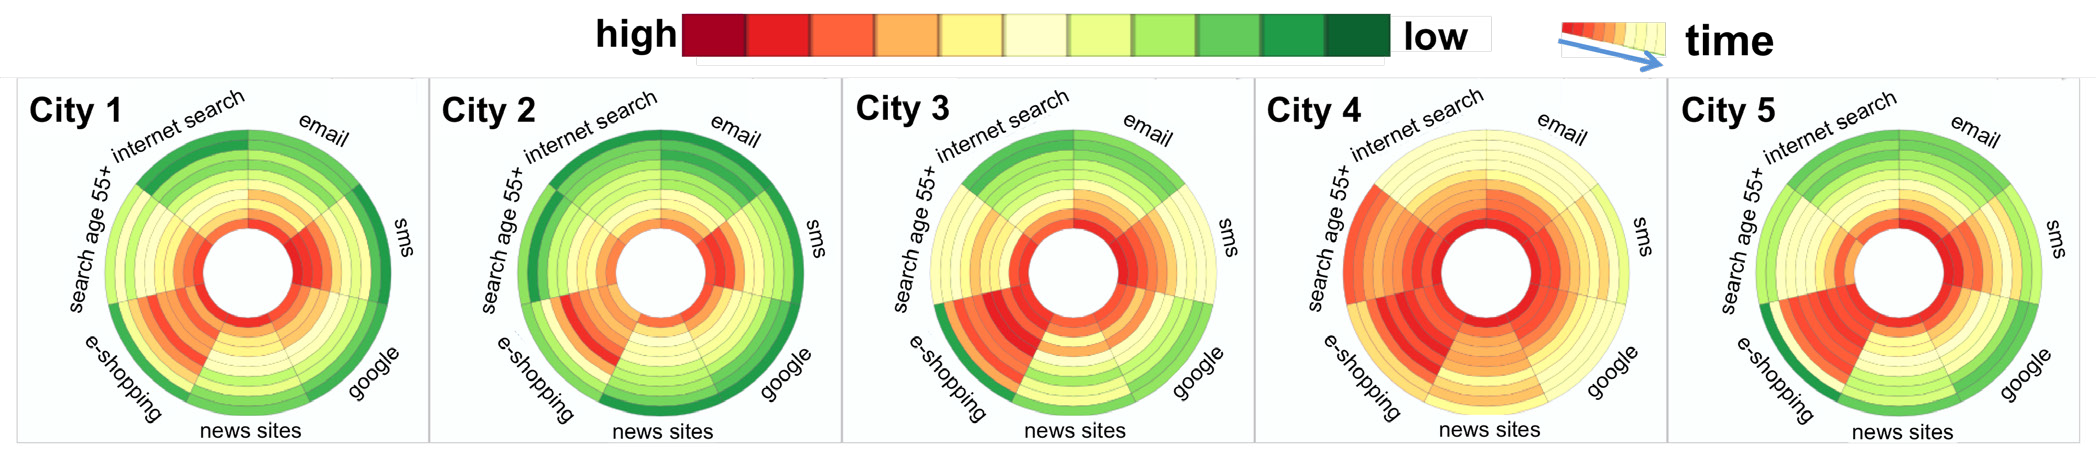
\includegraphics[width=\textwidth]{figs/circle.png}
\end{frame}

\section{Categorical Keys and Quantitative Values}
\frame{\sectionpage}

\begin{frame}{UpSet\cite{lex_upset:_2014}}
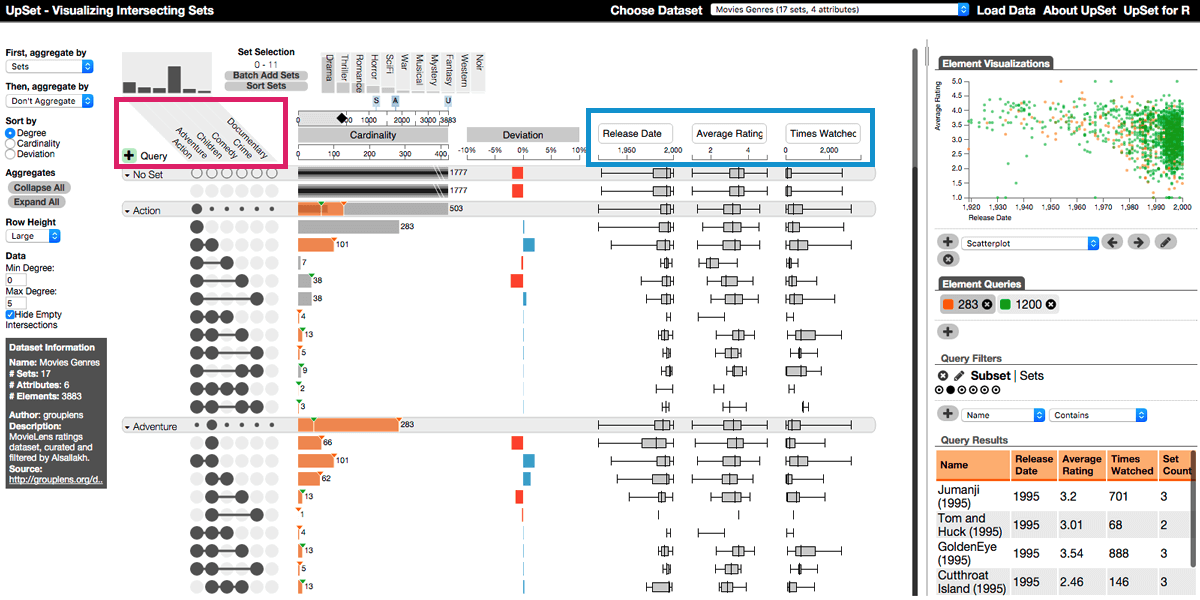
\includegraphics[width=\textwidth]{figs/2014_infovis_upset_teaser.png}
\end{frame}


\begin{frame}{Flexible Axes\cite{claessen_flexible_2011}}
\begin{figure}
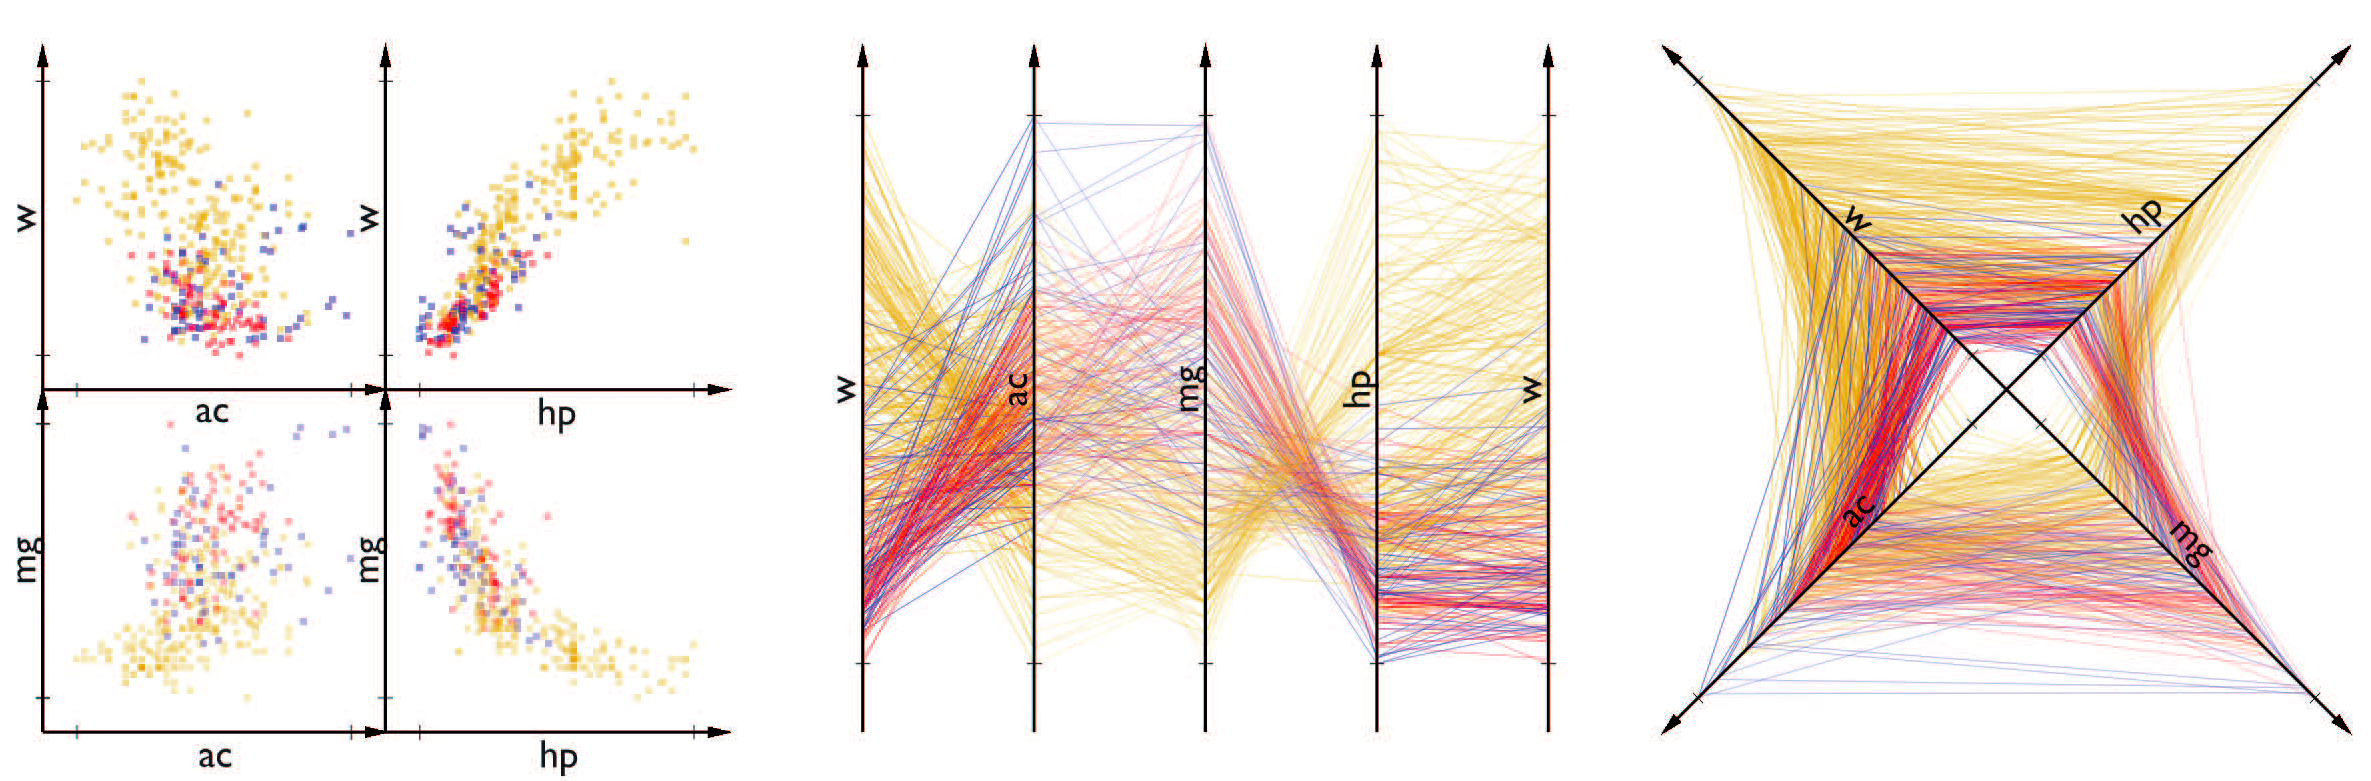
\includegraphics[width=\textwidth]{figs/flexaxis.png}
\end{figure}
\begin{description}
        \item[values] ac = acceleration, mg = miles per gallon, w = weight, hp = horse power, yr = model year, cy = cylinders, and dp = displacement
        \item[keys] country of origin: USA (yellow), Europe(blue), Japan (red)
\end{description}
\end{frame}


\section{Quantitative Keys and Categorical Values}
\frame{\sectionpage}

\begin{frame}{Streamgraph\cite{byron_stacked_2008}}
\begin{figure}
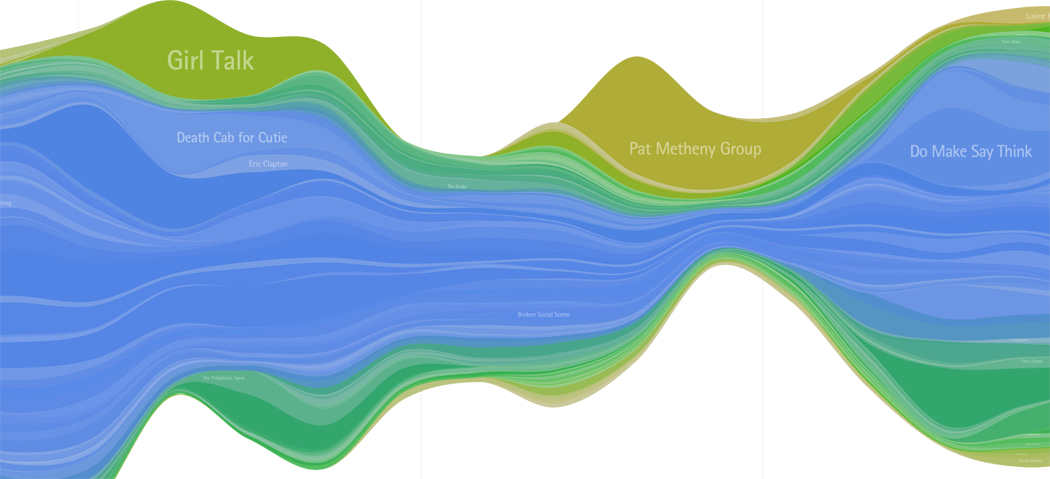
\includegraphics[width=\textwidth]{figs/stream.png}
\end{figure}
\begin{description}
        \item[values] musical trends
        \item[key] timeseries
\end{description}

\end{frame}


\section{Quantitative Keys and Quantitative Values}
\frame{\sectionpage}

\begin{frame}{Partial Dependence Plots\cite{_elements_2009}}
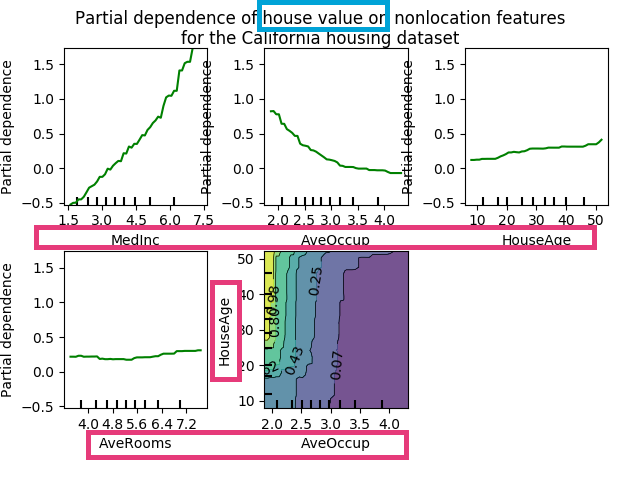
\includegraphics[width=\textwidth]{figs/partial_dependence.png}

\end{frame}

\begin{frame}{Cluster \& Calendar\cite{van_wijk_cluster_1999}}
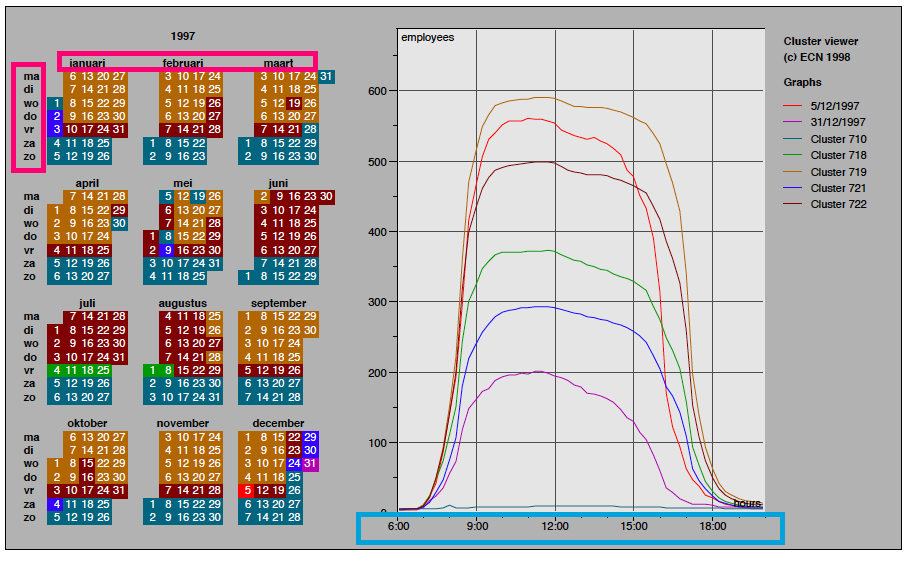
\includegraphics[width=\textwidth]{figs/calendar.png}
\end{frame}

\begin{frame}{Bivariate Colormaps\cite{lucchesi_visualizing_2017}}
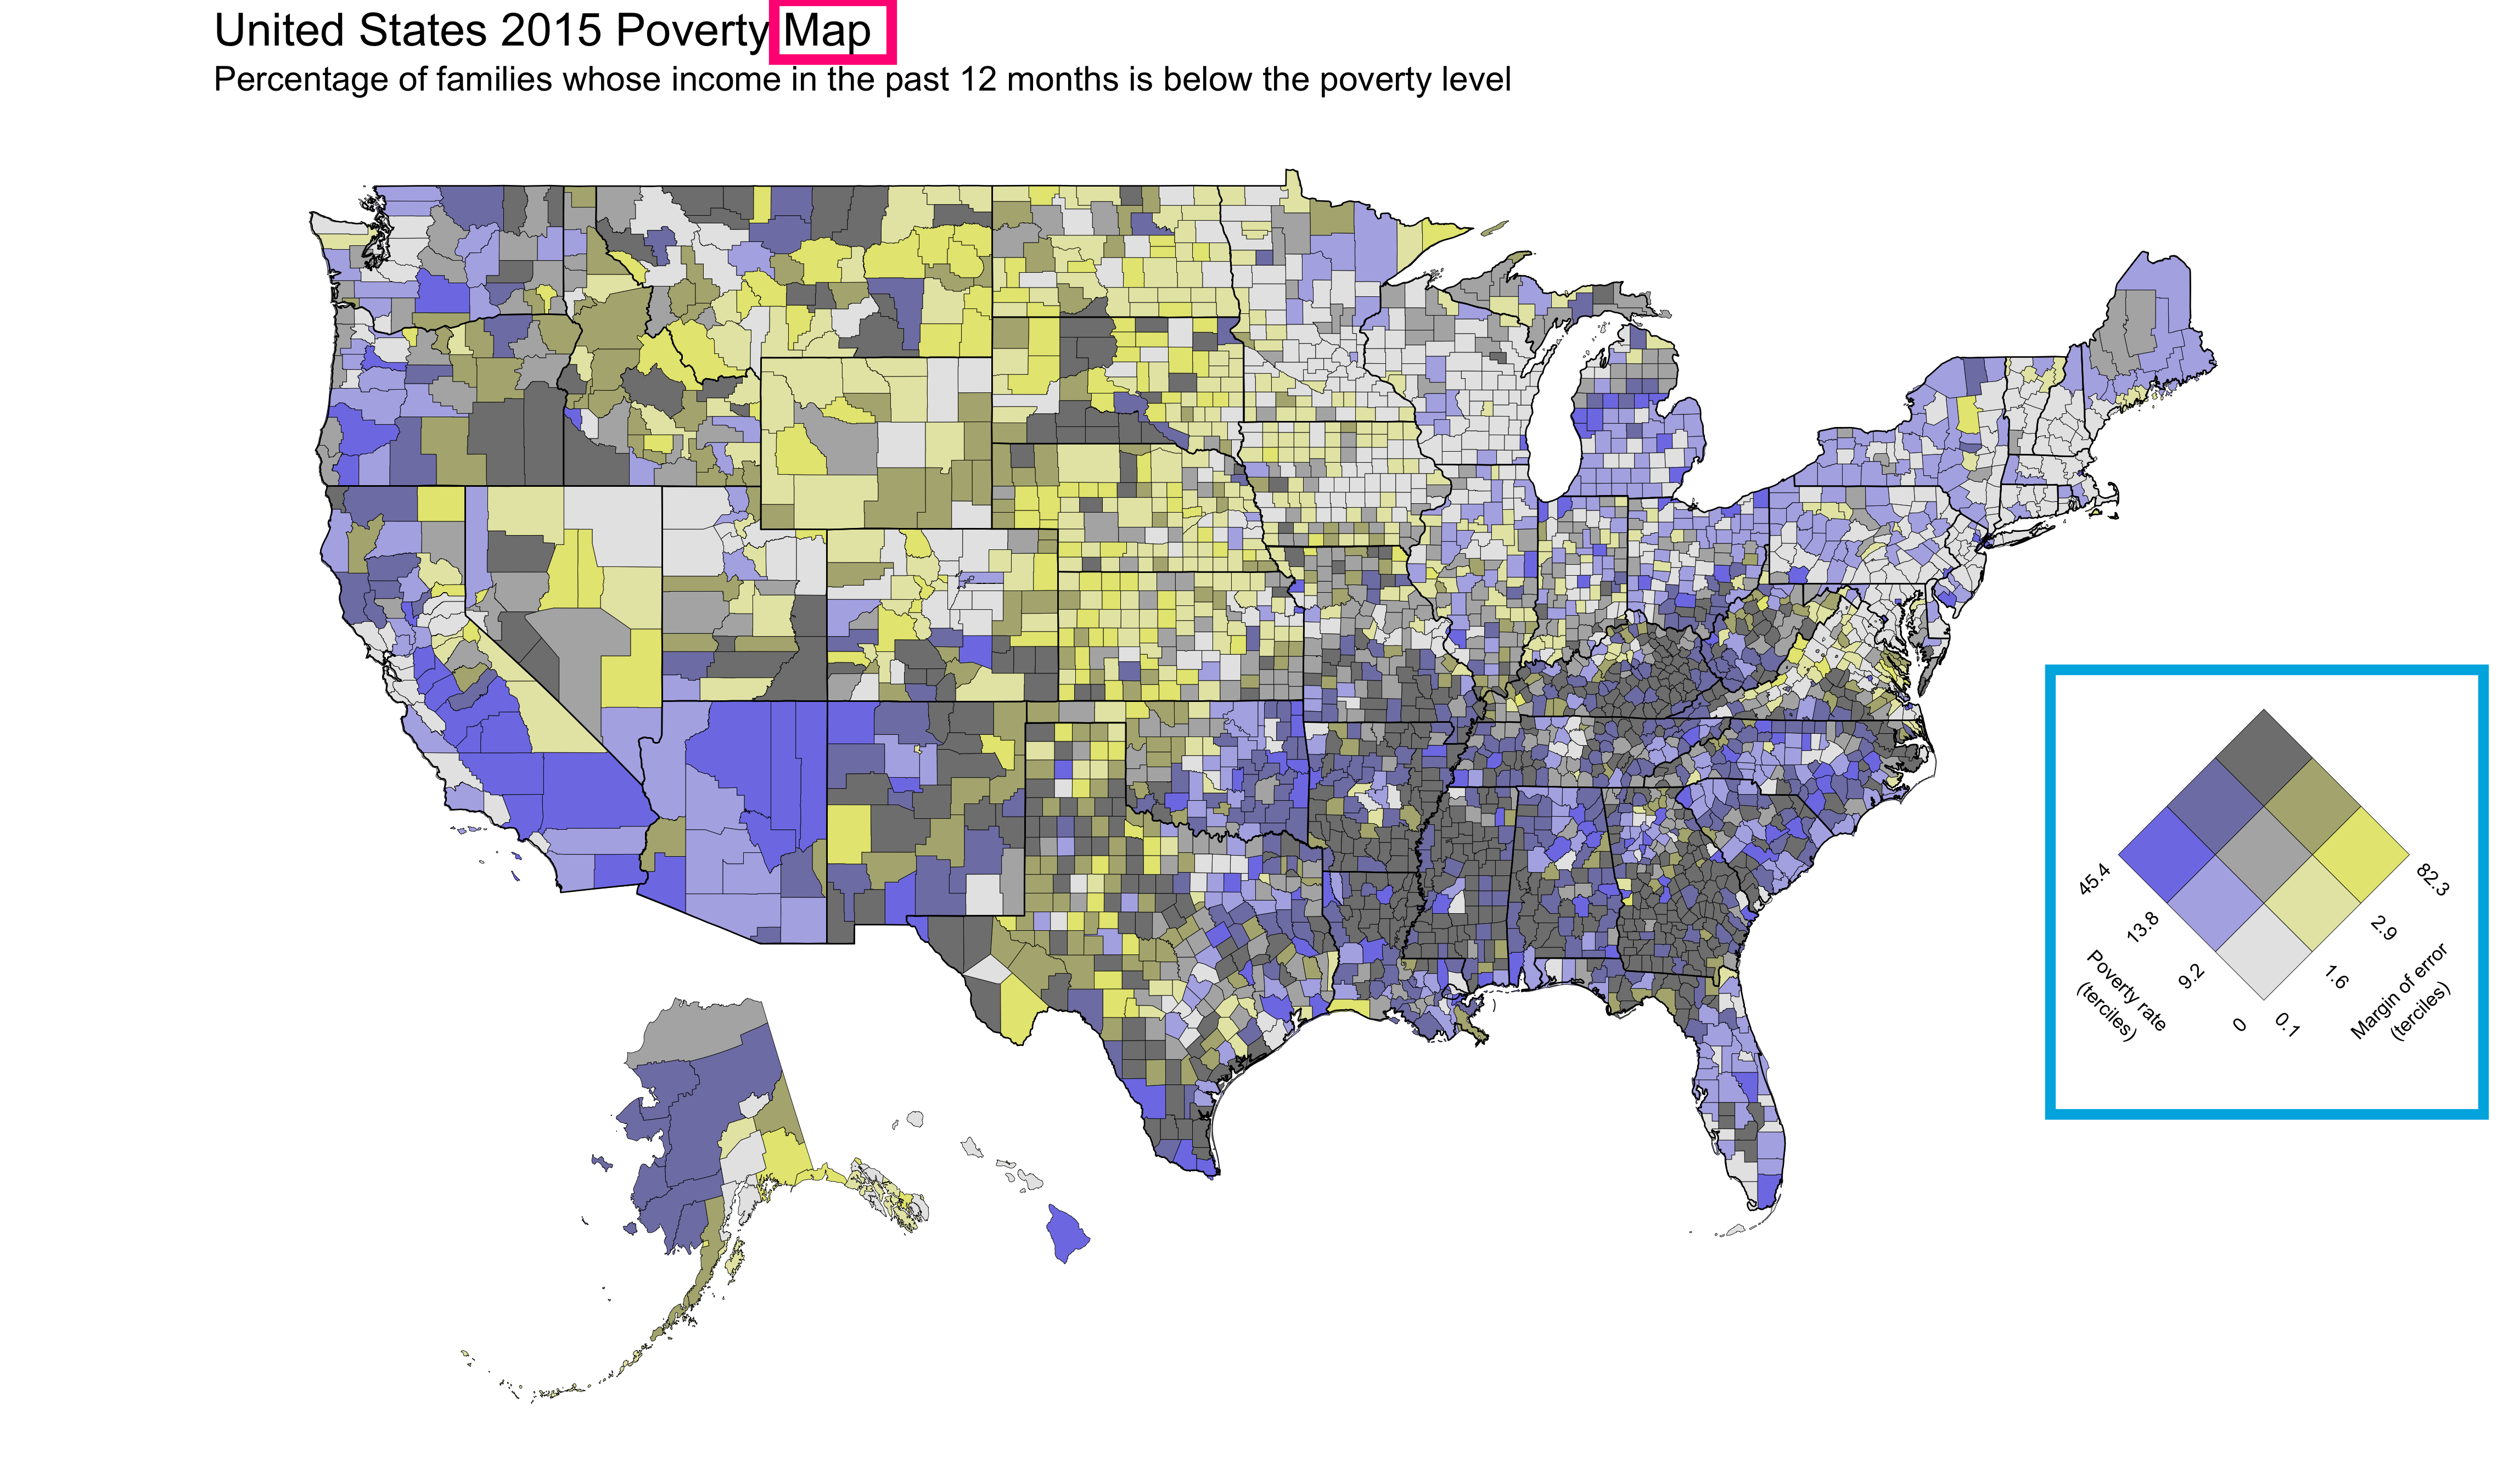
\includegraphics[width=\textwidth]{figs/bivariate_anotated.png}
\end{frame}


\section{Functional Values}
\frame{\sectionpage}

\begin{frame}{Contour Boxplots\cite{whitaker_contour_2013}}
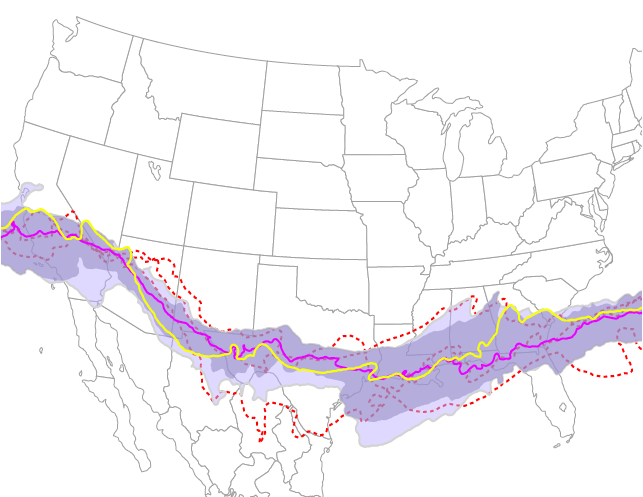
\includegraphics[height=.75\textheight]{figs/contour_weather.png}
\end{frame}

\begin{frame}{Surface Boxplots\cite{genton_surface_2014}}
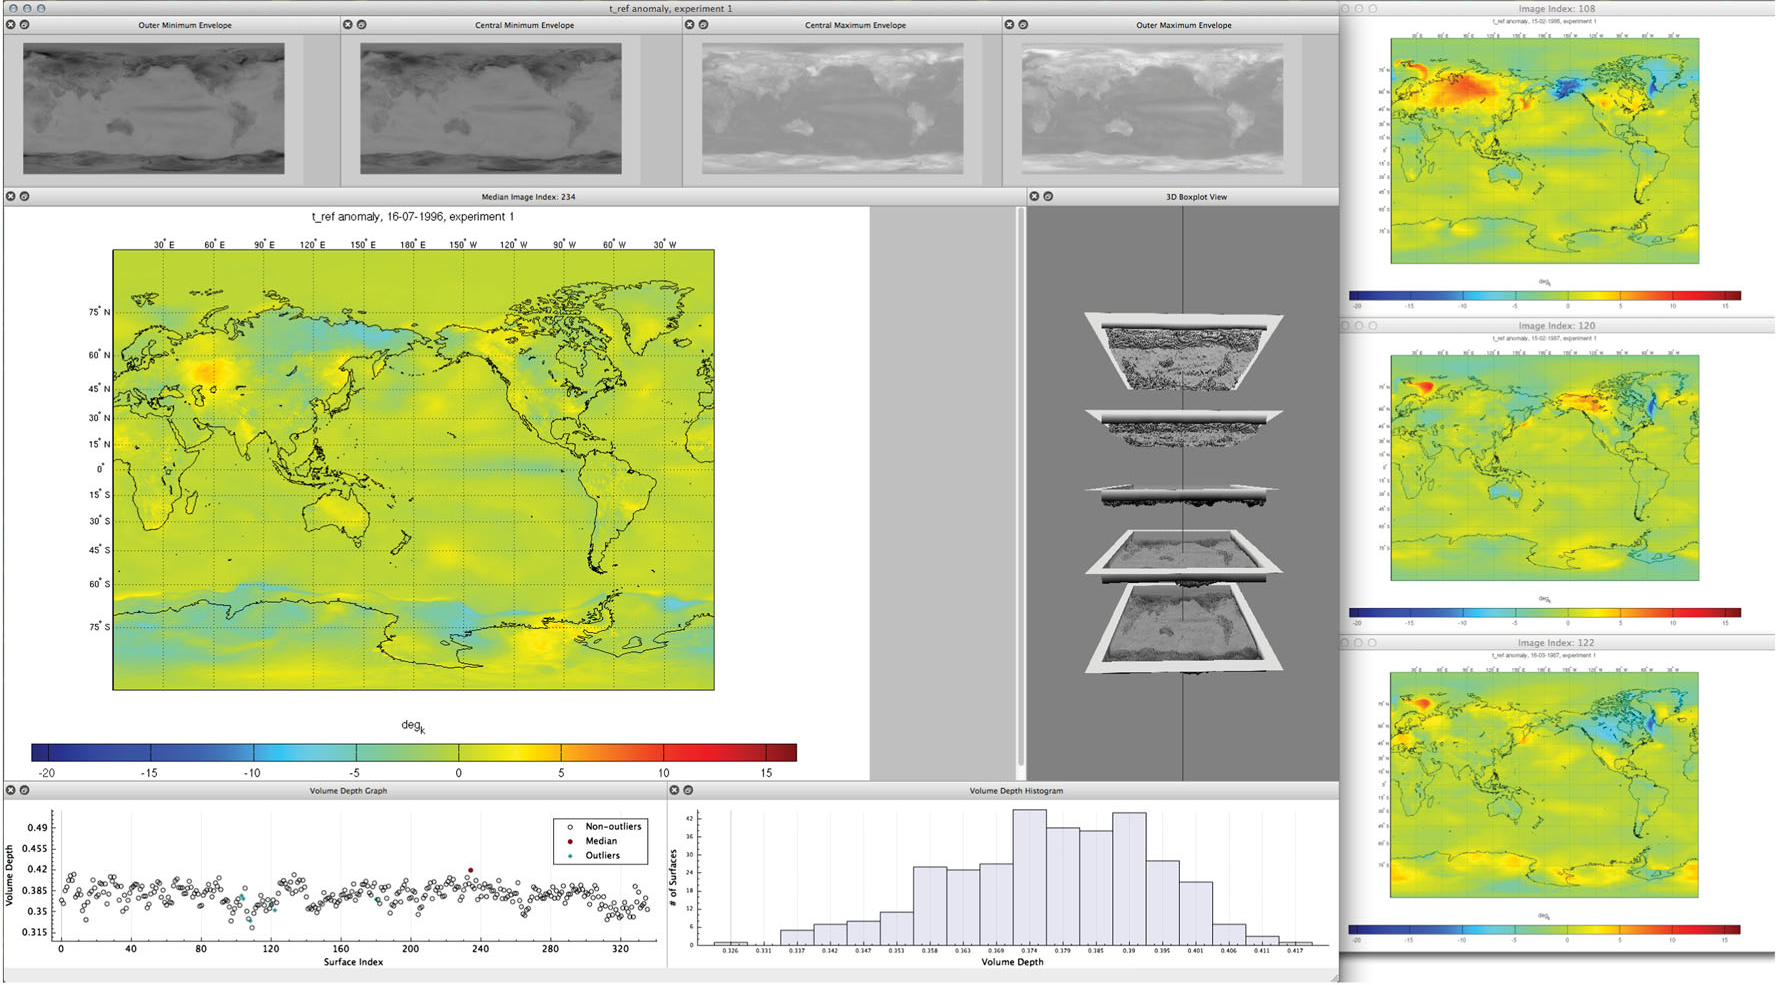
\includegraphics[width=\textwidth]{figs/surfacebox.png}
\end{frame}

\section{Conclusion}
\begin{frame}{Conclusion}
\begin{enumerate}
    \item Densities and distributions are important
    \item Visualization methods fall off as variables get more complex
    \item Can we build on current methods to show conditional dependencies and functional variables? 
\end{enumerate}
\end{frame}

\begin{frame}[allowframebreaks]{References}
\printbibliography
\end{frame}
\end{document}

